\documentclass[12pt]{article}
\usepackage[top=3cm, left=3cm, right=3cm, bottom=2.5cm]{geometry}
\usepackage{amsmath,bm}
\usepackage{xcolor}
\usepackage{float}
\usepackage{graphicx}
\usepackage{nicefrac}
\usepackage{amsfonts}


\begin{document}

\title{Fiber circuits - E.Coli}
\author{Higor S. Monteiro}

\maketitle

% SECTION 1
\section{Circuits $|n=0, \ell \rangle$}

\begin{figure}[H]
    \centering
    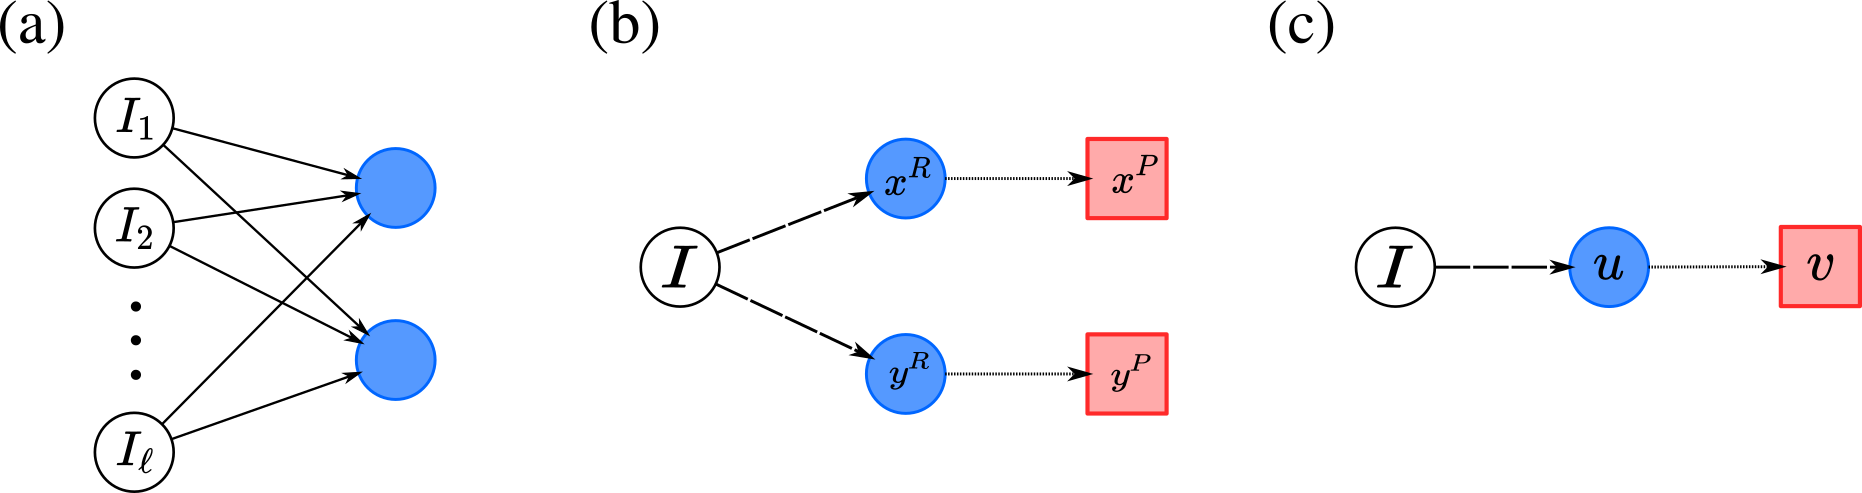
\includegraphics[scale=0.5]{figs/n0l_1.png}
    \caption{(a) Biological representation, 
        (b) Mathematical representation, and (c) quotient
        network.}
    \label{fig:fig1}
\end{figure}

\subsection{General admissible equations}

\begin{equation} \label{eq:n0_gen_eq}
    \begin{aligned}
        \dot{x}^R &= f(x^R, I)\\
        \dot{x}^P &= g(x^P, x^R)\\
        \dot{y}^R &= f(y^R, I)\\
        \dot{y}^P &= g(y^P, y^R),
    \end{aligned}
\end{equation}
with vector of coordinates $\vec{x} = (x^R, x^P, y^R, y^P)$.

\subsection{Jacobian and eigenvalues}

Considering the partial derivatives obtained from 
Eq.~\ref{eq:n0_gen_eq}, we have:
$\nicefrac{\partial \dot{x}^R}{\partial {x}^R} = f_1$;
$\nicefrac{\partial \dot{x}^P}{\partial {x}^R} = g_2$;
$\nicefrac{\partial \dot{x}^P}{\partial {x}^P} = g_1$;
$\nicefrac{\partial \dot{y}^R}{\partial {x}^R} = f_1$;
$\nicefrac{\partial \dot{y}^P}{\partial {x}^P} = g_1$;
$\nicefrac{\partial \dot{y}^P}{\partial {y}^R} = g_2$.
From these derivatives at the equilibrium point, the 
Jacobian is given as
\begin{equation}
    J = \begin{pmatrix}
        f_1 & 0 & 0 & 0 \\
        g_2 & g_1 & 0 & 0 \\
        0 & 0 & f_1 & 0 \\
        0 & 0 & g_2 & g_1 \\
    \end{pmatrix}_{\big|_{eq.}} =
    \begin{pmatrix}
        a & 0 & 0 & 0 \\
        c & b & 0 & 0 \\
        0 & 0 & a & 0 \\
        0 & 0 & c & b \\ 
    \end{pmatrix}.
\end{equation}

Eigenvalues of $J$:

$\lambda_1 = a$, $\lambda_2 = a$, $\lambda_3 = b$, 
$\lambda_4 = b$\\

Eigenvectors of $J$:

$ v_1 = \Big( 0, 0, \frac{a-b}{c}, 1 \Big)$

$ v_2 = \Big( \frac{a-b}{c}, 1, 0, 0 \Big)$

$ v_3 = \Big( 0, 0, 0, 1 \Big)$

$ v_4 = \Big( 0, 1, 0, 0 \Big)$

\subsection{Realizations in E. coli}

\begin{figure}[H]
    \centering
    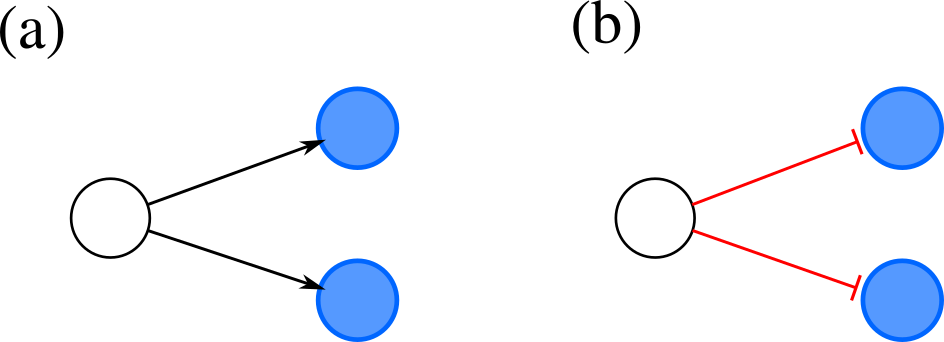
\includegraphics[scale=0.5]{figs/n0l1_ecoli.png}
    \caption{$|n=0, \ell = 1\rangle$}
    \label{fig:fig1_l1}
\end{figure}

\begin{figure}[H]
    \centering
    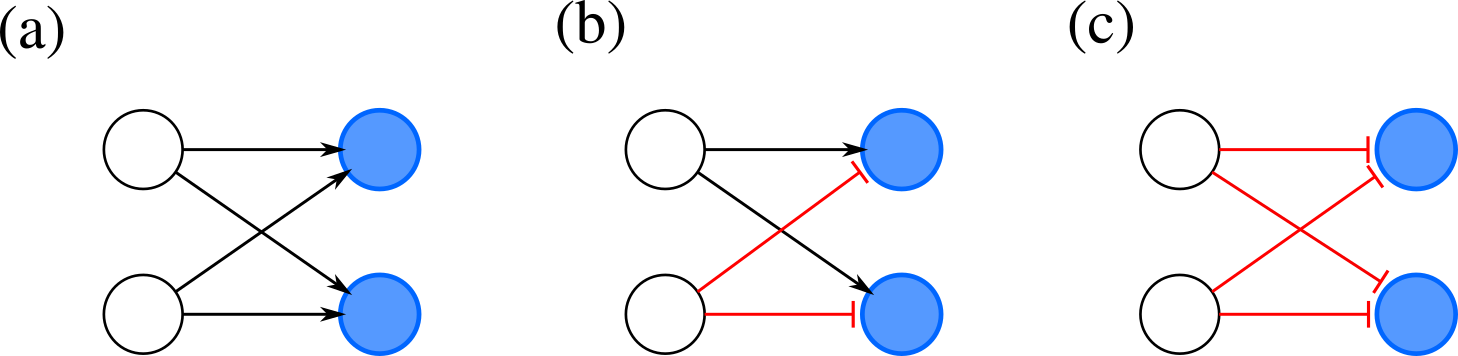
\includegraphics[scale=0.5]{figs/n0l2_ecoli.png}
    \caption{$|n=0, \ell = 2\rangle$}
    \label{fig:fig1_l2}
\end{figure}

\begin{figure}[H]
    \centering
    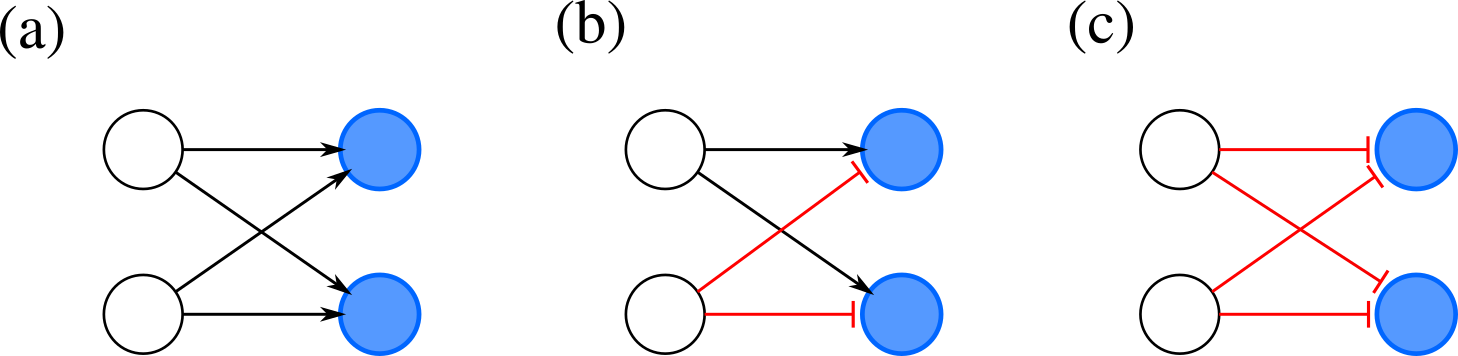
\includegraphics[scale=0.5]{figs/n0l2_ecoli.png}
    \caption{$|n=0, \ell = 3\rangle$}
    \label{fig:fig1_l2}
\end{figure}

\subsection{Special model}

Since all inputs $I_1, I_2, \dots, I_{\ell}$ are
symmetric, then we can represent all them by 
$I = \sum_j^{\ell} I_j$, which preserves the symmetry.
Therefore, the special model for all circuits above
is given by
\begin{equation}
    \begin{aligned}
        f(u, I) &= -\alpha u + I\\
        g(u, v) &= -\delta u + \beta v
    \end{aligned},
\end{equation}
where we can observe that $I$ cannot act as a bifurcation
parameter.

\subsection{Bifurcation conditions}

Performing the partial derivatives on the special model
we obtain that
\begin{equation}
    \dfrac{\partial f}{\partial u} = -\alpha; \ \ 
    \dfrac{\partial g}{\partial u} = -\delta; \ \
    \dfrac{\partial g}{\partial v} = \beta, 
\end{equation}
for which we have
\begin{equation}
    \lambda_{1,2} = -\alpha < 0; \ \ 
    \lambda_{3,4} = -\delta <0.
\end{equation}
In this case, we expect synchrony-preserving
($\lambda_{1,2} < 0$) 
bifurcations, but no oscillations 
($\lambda_{3,4} < 0$).

\section{Circuits $|n=1, \ell \rangle$}

\begin{figure}[H]
    \centering
    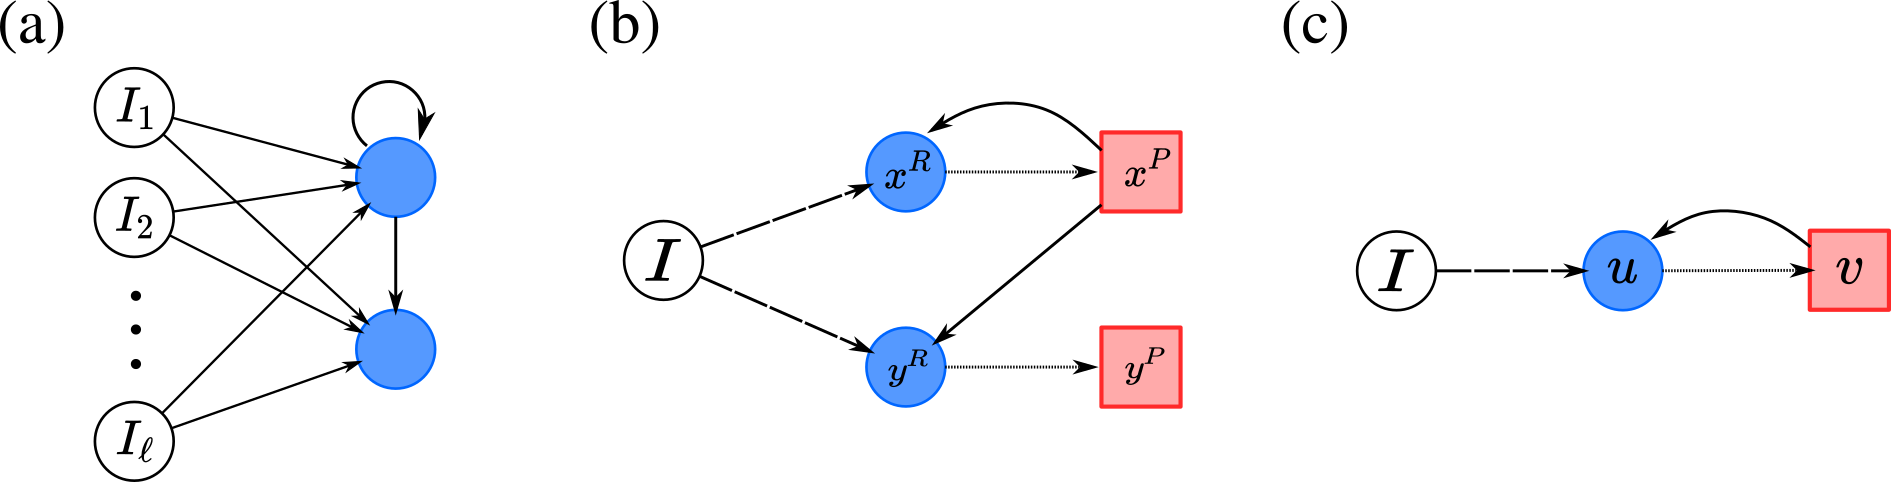
\includegraphics[scale=0.5]{figs/n1l_1.png}
    \caption{(a) Biological representation, 
        (b) Mathematical representation, and (c) quotient
        network.}
    \label{fig:fig2}
\end{figure}

\subsection{General admissible equations}

\begin{equation} \label{eq:n1_gen_eq}
    \begin{aligned}
        \dot{x}^R &= f(x^R, x^P, I)\\
        \dot{x}^P &= g(x^P, x^R)\\
        \dot{y}^R &= f(y^R, x^P, I)\\
        \dot{y}^P &= g(y^P, y^R),
    \end{aligned}
\end{equation}
with vector of coordinates $\vec{x} = (x^R, x^P, y^R, y^P)$.

\subsection{Jacobian and eigenvalues}

Considering the partial derivatives obtained from 
Eq.~\ref{eq:n1_gen_eq}, we have:
$\nicefrac{\partial \dot{x}^R}{\partial {x}^R} = f_1$,
$\nicefrac{\partial \dot{x}^R}{\partial {x}^P} = f_2$,
$\nicefrac{\partial \dot{x}^P}{\partial {x}^R} = g_2$,
$\nicefrac{\partial \dot{x}^P}{\partial {x}^P} = g_1$,
$\nicefrac{\partial \dot{y}^R}{\partial {x}^R} = f_1$,
$\nicefrac{\partial \dot{y}^R}{\partial {x}^P} = f_2$,
$\nicefrac{\partial \dot{y}^P}{\partial {x}^P} = g_1$,
$\nicefrac{\partial \dot{y}^P}{\partial {y}^R} = g_2$,
From these derivatives at the equilibrium point, the 
Jacobian is given as
\begin{equation}
    J = \begin{pmatrix}
        f_1 & f_2 & 0 & 0 \\
        g_2 & g_1 & 0 & 0 \\
        0 & f_2 & f_1 & 0 \\
        0 & 0 & g_2 & g_1 \\
    \end{pmatrix}_{\big|_{eq.}} =
    \begin{pmatrix}
        a & b & 0 & 0 \\
        d & c & 0 & 0 \\
        0 & b & a & 0 \\
        0 & 0 & d & c \\ 
    \end{pmatrix}
\end{equation}

Eigenvalues of $J$:

$\lambda_1 = a$, $\lambda_2 = c$, 
$\lambda_{3,4} = \frac{1}{2}(a+c \mp \sqrt{(a-c)^2 + 4bd})$\\[0.2cm]

Eigenvectors of $J$:

$ v_1 = \Big( 0, 0, \frac{a-c}{d}, 1 \Big)$

$ v_2 = \Big( 0, 0, 0, 1 \Big)$

$ v_3 = \Big( -\frac{(-a + c + \sqrt{(a-c)^2 + 4bd})}{2d}, 
        1, -\frac{(-a + c + \sqrt{(a-c)^2 + 4bd})}{2d}, 1 \Big)$

$ v_4 = \Big( -\frac{(-a + c - \sqrt{(a-c)^2 + 4bd})}{2d}, 
        1, -\frac{(-a + c - \sqrt{(a-c)^2 + 4bd})}{2d}, 1 \Big)$\\[0.2cm]

\subsection{Realizations in E. coli}

\begin{figure}[H]
    \centering
    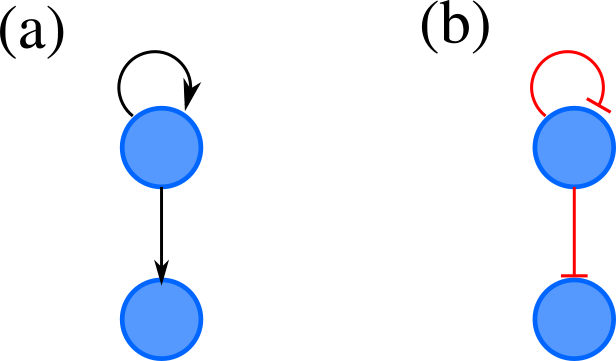
\includegraphics[scale=0.5]{figs/n1l0_ecoli.png}
    \caption{$|n=1, \ell = 0\rangle$}
    \label{fig:fig2_l0}
\end{figure}

\begin{figure}[H]
    \centering
    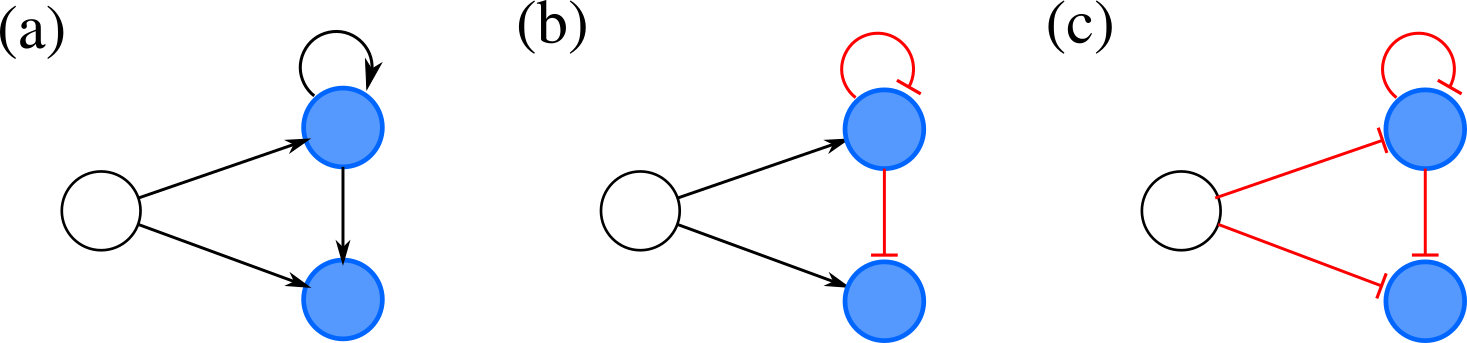
\includegraphics[scale=0.5]{figs/n1l1_ecoli.png}
    \caption{$|n=1, \ell = 1\rangle$}
    \label{fig:fig2_l1}
\end{figure}

\begin{figure}[H]
    \centering
    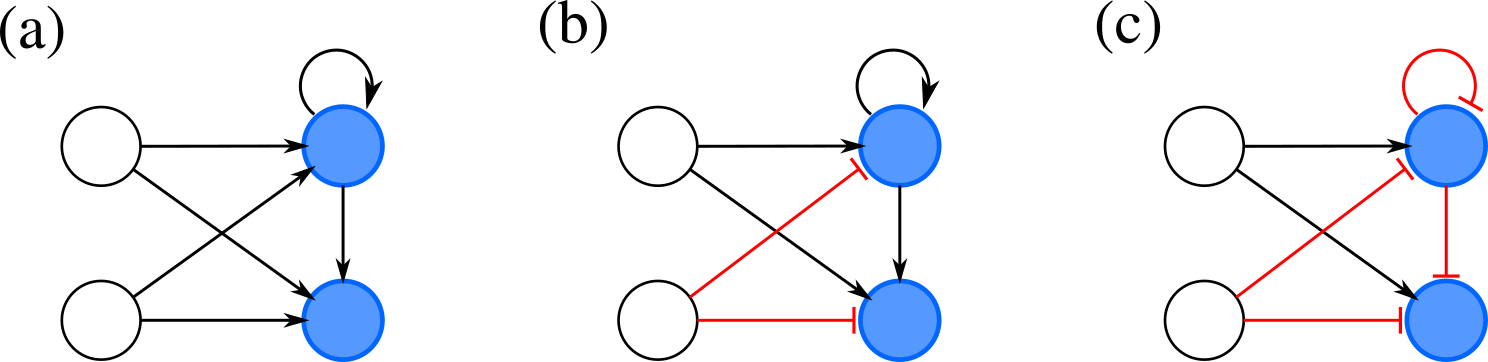
\includegraphics[scale=0.5]{figs/n1l2_ecoli.png}
    \caption{$|n=1, \ell = 2\rangle$}
    \label{fig:fig2_l2}
\end{figure}

\subsection{Special model}

Regarding the inputs $I_1, I_2, \dots, I_{\ell}$
we know that they must be symmetric in order to keep
the fibration symmetry. Therefore, we represent all
the inputs by $I = \sum_j^{\ell} I_j$, which should
preserve the symmetry. Now, considering the special
model for the circuits above, we have two cases:\\[0.2cm]

1. UNSAT-FFF Circuits: Fig.~\ref{fig:fig2_l0}(b), 
Fig.~\ref{fig:fig2_l1}(b) and (c), and 
Fig.~\ref{fig:fig2_l2}(c).
\begin{equation}
    \begin{aligned}
        f(u, v, I) &= -\alpha u + S(v) +  I\\
        g(u, v) &= -\delta u + \beta v
    \end{aligned}
\end{equation}
\\[0.2cm]

2. SAT-FFF Circuits: Fig.~\ref{fig:fig2_l0}(a), 
Fig.~\ref{fig:fig2_l1}(a), and 
Fig.~\ref{fig:fig2_l2}(a) and (b).
\begin{equation}
    \begin{aligned}
        f(u, v, I) &= -\alpha u + (1 - S(v)) +  I\\
        g(u, v) &= -\delta u + \beta v
    \end{aligned},
\end{equation}
where in both cases $I$ cannot act as bifurcation 
parameter.


\subsection{Bifurcation conditions}

Performing the partial derivatives on the special models
above we obtain that for case 1
\begin{equation}
    \dfrac{\partial f}{\partial u} = -\alpha; \ \
    \dfrac{\partial f}{\partial v} = S'(v) < 0; \ \ 
    \dfrac{\partial g}{\partial u} = -\delta; \ \
    \dfrac{\partial g}{\partial v} = \beta, 
\end{equation}
for which we have
\begin{equation}
    a = -\alpha = \lambda_1; \ \ 
    b = S'(v); \ \ 
    c = -\delta = \lambda_2; \ \ 
    d = \beta.
\end{equation}
In this case, we expect synchrony-preserving
($\lambda_{1,2} < 0$) 
bifurcations, and decaying oscillations since
$\lambda_{3,4}$ are complex with negative real parts. If $a + c \approx 0$,
we have approximately stable oscillations.

For case 2, we have
\begin{equation}
    \dfrac{\partial f}{\partial u} = -\alpha; \ \
    \dfrac{\partial f}{\partial v} = -S'(v) > 0; \ \ 
    \dfrac{\partial g}{\partial u} = -\delta; \ \
    \dfrac{\partial g}{\partial v} = \beta, 
\end{equation}
for which we have
\begin{equation}
    a = -\alpha = \lambda_1; \ \ 
    b = -S'(v); \ \ 
    c = -\delta = \lambda_2; \ \ 
    d = \beta.
\end{equation}
In this case, we expect synchrony-preserving
($\lambda_{1,2} < 0$) 
bifurcations, but no oscillations since 
$(a-c)^2 + 4bd$ is positive.

\section{Circuits $|n = 2, \ell \rangle$}

\begin{figure}[H]
    \centering
    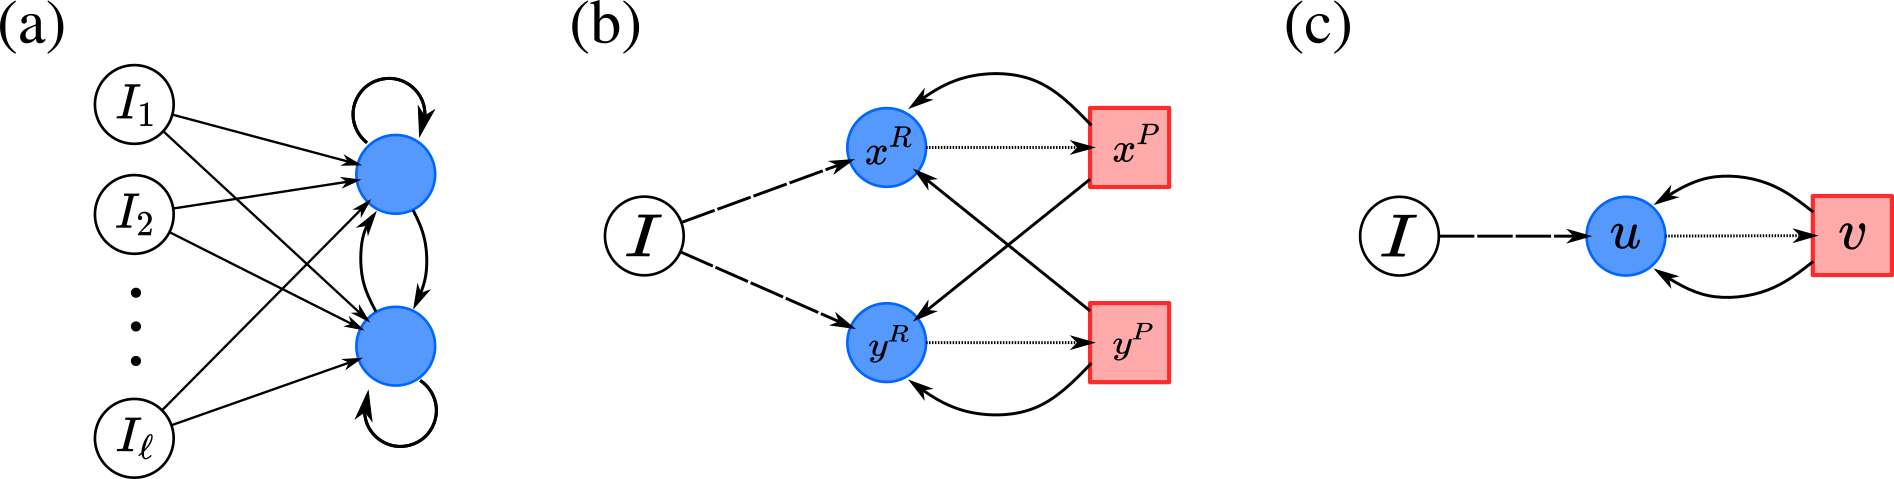
\includegraphics[scale=0.5]{figs/n2l_1.png}
    \caption{(a) Biological representation, 
        (b) Mathematical representation, and (c) quotient
        network.}
    \label{fig:fig3}
\end{figure}

\subsection{General admissible equations}

\begin{equation} \label{eq:n2_gen_eq}
    \begin{aligned}
        \dot{x}^R &= f(x^R, \overline{x^P, y^P}, I)\\
        \dot{x}^P &= g(x^P, x^R)\\
        \dot{y}^R &= f(y^R, \overline{x^P, y^P}, I)\\
        \dot{y}^P &= g(y^P, y^R),
    \end{aligned}
\end{equation}
Obs: The bar $\overline{x^P, y^P}$ representing the vertex 
symmetry is only valid when all regulations are 
of the same type.

\subsection{Jacobian and eigenvalues}

Considering the partial derivatives obtained from 
Eq.~\ref{eq:n2_gen_eq}, we have:
$\nicefrac{\partial \dot{x}^R}{\partial {x}^R} = f_1$,
$\nicefrac{\partial \dot{x}^R}{\partial {x}^P} = f_2$,
$\nicefrac{\partial \dot{x}^R}{\partial {y}^P} = f_3$,
$\nicefrac{\partial \dot{x}^P}{\partial {x}^R} = g_2$,
$\nicefrac{\partial \dot{x}^P}{\partial {x}^P} = g_1$,
$\nicefrac{\partial \dot{y}^R}{\partial {x}^R} = f_1$,
$\nicefrac{\partial \dot{y}^R}{\partial {x}^P} = f_2$,
$\nicefrac{\partial \dot{y}^R}{\partial {y}^P} = f_3$,
$\nicefrac{\partial \dot{y}^P}{\partial {x}^P} = g_1$,
$\nicefrac{\partial \dot{y}^P}{\partial {y}^R} = g_2$.
From these derivatives at the equilibrium point, the 
Jacobian is given as
\begin{equation}
    J = \begin{pmatrix}
        f_1 & f_2 & 0 & f_3 \\
        g_2 & g_1 & 0 & 0 \\
        0 & f_2 & f_1 & f_3 \\
        0 & 0 & g_2 & g_1 \\
    \end{pmatrix}_{\big|_{eq.}} =
    \begin{pmatrix}
        a & b & 0 & c \\
        e & d & 0 & 0 \\
        0 & b & a & c \\
        0 & 0 & e & d \\ 
    \end{pmatrix}
\end{equation}\\[0.2cm]

Eigenvalues of $J$:

$\lambda_1 = a$, $\lambda_2 = d$, 
$\lambda_{3,4} = \frac{1}{2}(a+d \mp \sqrt{(a-d)^2 + 4e(b+c)})$\\[0.2cm]

Eigenvectors of $J$:

$ v_1 = \Big( \frac{c(d-a)}{be}, -\frac{c}{b}, \frac{a-d}{e}, 1 \Big)$

$ v_2 = \Big( 0, -\frac{c}{b}, 0, 1 \Big)$

$ v_3 = \Big( -\frac{(d - a + \sqrt{(a-d)^2 + 4e(b+c)})}{2e}, 
        1, -\frac{(d - a + \sqrt{(a-d)^2 + 4e(b+c)})}{2e}, 1 \Big)$\\[0.2cm]

$ v_4 = \Big( -\frac{(d - a - \sqrt{(a-d)^2 + 4e(b+c)})}{2e}, 
        1, -\frac{(d - a - \sqrt{(a-d)^2 + 4e(b+c)})}{2e}, 1 \Big)$\\[0.2cm]

Obs: When all regulations are the same, then $f_2 = f_3$ at the equilibrium due 
to the vertex symmetry.

\subsection{Realizations in E. coli}

\begin{figure}[H]
    \centering
    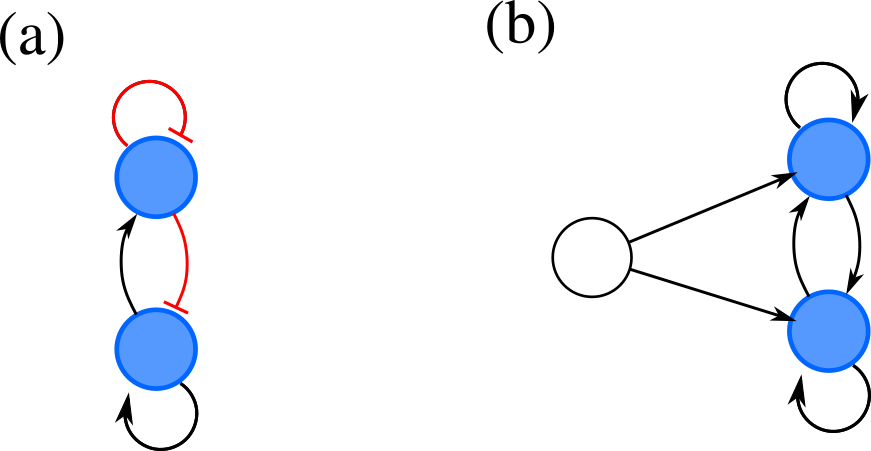
\includegraphics[scale=0.5]{figs/n2l0l1_ecoli.png}
    \caption{(a) $|n=2,\ell = 0\rangle$. (b) $|n=2, \ell=1\rangle$}
    \label{fig:fig3_l0l1}
\end{figure}

\subsection{Special model}

Following Prof. Ian's notes, we have for 
Fig.~\ref{fig:fig3_l0l1}(a)
\begin{equation}
    \begin{aligned}
        f(u, v, w, I) &= -\alpha u + 1-S(v) +  T(w)\\
        g(u, v) &= -\delta u + \beta v
    \end{aligned},
\end{equation}
where $S(v)$ and $T(w)$ are both Hill functions.

For Fig.~\ref{fig:fig3_l0l1}(b) we have
\begin{equation}
    \begin{aligned}
        f(u, v, w, I) &= -\alpha u + (1 - S(v)) +  (1-S(w))\\
        g(u, v) &= -\delta u + \beta v
    \end{aligned}
\end{equation}

\subsection{Bifurcation conditions}

Performing the partial derivatives on the special models
above we obtain for Fig.~\ref{fig:fig3_l0l1}(a) that 
\begin{equation}
    \dfrac{\partial f}{\partial u} = -\alpha; \ \
    \dfrac{\partial f}{\partial v} = -S'(v) > 0; \ \
    \dfrac{\partial f}{\partial w} = T'(w) < 0; \ \ 
    \dfrac{\partial g}{\partial u} = -\delta; \ \
    \dfrac{\partial g}{\partial v} = \beta, 
\end{equation}
for which we have
\begin{equation}
    a = -\alpha = \lambda_1; \ \ 
    b = -S'(v); \ \
    c = T'(w); \ \  
    d = -\delta = \lambda_2; \ \ 
    e = \beta.
\end{equation}
In this case, we expect synchrony-preserving
($\lambda_{1,2} < 0$) 
bifurcations, and decaying oscillations depending
on the magnitude of $c$. For these oscillations, they
are approximately stable if $a + d \approx 0$.

For Fig.~\ref{fig:fig3_l0l1}(b), we have
\begin{equation}
    \dfrac{\partial f}{\partial u} = -\alpha; \ \
    \dfrac{\partial f}{\partial v} = -S'(v) > 0; \ \
    \dfrac{\partial f}{\partial w} = -S'(w) > 0; \ \ 
    \dfrac{\partial g}{\partial u} = -\delta; \ \
    \dfrac{\partial g}{\partial v} = \beta, 
\end{equation}
for which we have
\begin{equation}
    a = -\alpha = \lambda_1; \ \ 
    b = c = -S'(v); \ \
    d = -\delta = \lambda_2; \ \ 
    e = \beta.
\end{equation}
In this case, we expect synchrony-preserving
($\lambda_{1,2} < 0$) 
bifurcations, but no oscillations since 
$(a-d)^2 + 4e(b+c)$ is positive.

\section{2-Fibo Fiber on $| n = 1, \ell = 2\rangle$ - Simple input}

\begin{figure}[H]
    \centering
    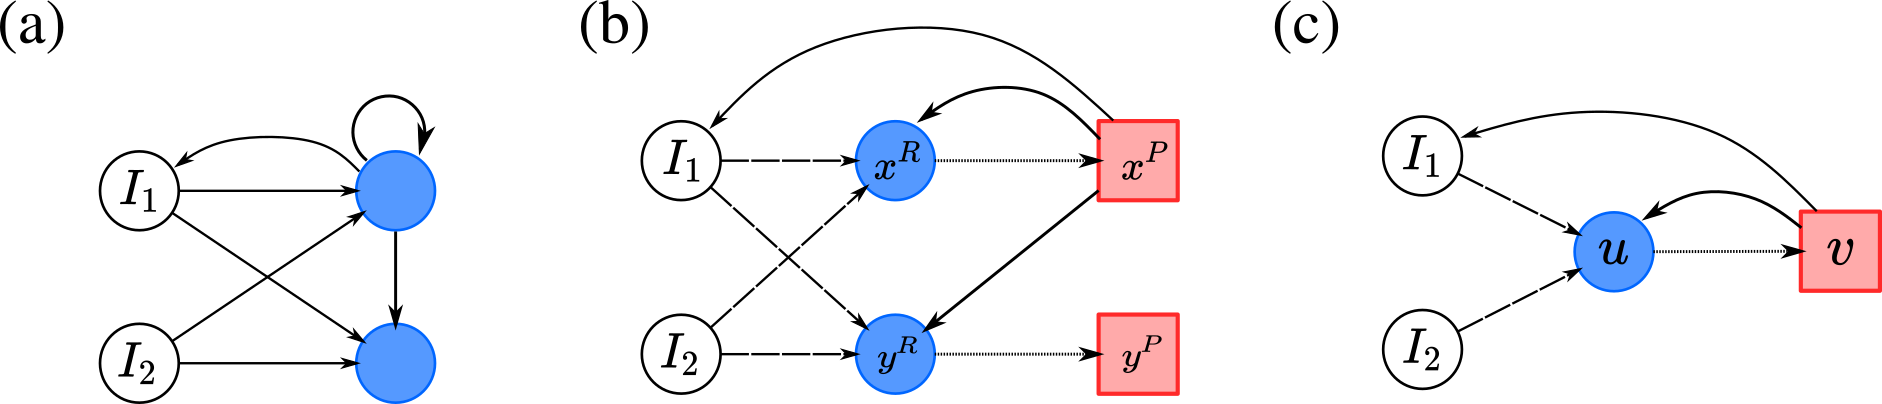
\includegraphics[scale=0.5]{figs/fibo2_simple.png}
    \caption{(a) Biological representation, 
        (b) Mathematical representation, and (c) quotient
        network.}
    \label{fig:fig4}
\end{figure}

\subsection{General admissible equations}
\begin{equation} \label{eq:2fibo-simple}
    \begin{aligned}
        \dot{x}^R &= f(x^R, x^P, I_1(x^P), I_2)\\
        \dot{x}^P &= g(x^P, x^R)\\
        \dot{y}^R &= f(y^R, x^P, I_1(x^P), I_2)\\
        \dot{y}^P &= g(y^P, y^R),
    \end{aligned}
\end{equation}
with vector of coordinates $\vec{x} = (x^R, x^P, y^R, y^P)$.

\subsection{Jacobian and eigenvalues}

Considering the partial derivatives obtained from 
Eq.~\ref{eq:2fibo-simple}, we have:
$\nicefrac{\partial \dot{x}^R}{\partial {x}^R} = f_1$,
$\nicefrac{\partial \dot{x}^R}{\partial {x}^P} = f_2$,
$\nicefrac{\partial \dot{x}^P}{\partial {x}^R} = g_2$,
$\nicefrac{\partial \dot{x}^P}{\partial {x}^P} = g_1$,
$\nicefrac{\partial \dot{y}^R}{\partial {x}^R} = f_1$,
$\nicefrac{\partial \dot{y}^R}{\partial {x}^P} = f_2$,
$\nicefrac{\partial \dot{y}^P}{\partial {x}^P} = g_1$,
$\nicefrac{\partial \dot{y}^P}{\partial {y}^R} = g_2$,
From these derivatives at the equilibrium point, the 
Jacobian is given as
\begin{equation}
    J = \begin{pmatrix}
        f_1 & f_2 & 0 & 0 \\
        g_2 & g_1 & 0 & 0 \\
        0 & f_2 & f_1 & 0 \\
        0 & 0 & g_2 & g_1 \\
    \end{pmatrix}_{\big|_{eq.}} =
    \begin{pmatrix}
        a & b & 0 & 0 \\
        d & c & 0 & 0 \\
        0 & b & a & 0 \\
        0 & 0 & d & c \\ 
    \end{pmatrix}
\end{equation}

Eigenvalues of $J$:

$\lambda_1 = a$, $\lambda_2 = c$, 
$\lambda_{3,4} = \frac{1}{2}(a+c \mp \sqrt{(a-c)^2 + 4bd})$\\[0.2cm]

Eigenvectors of $J$:

$ v_1 = \Big( 0, 0, \frac{a-c}{d}, 1 \Big)$

$ v_2 = \Big( 0, 0, 0, 1 \Big)$

$ v_3 = \Big( -\frac{(-a + c + \sqrt{(a-c)^2 + 4bd})}{2d}, 
        1, -\frac{(-a + c + \sqrt{(a-c)^2 + 4bd})}{2d}, 1 \Big)$

$ v_4 = \Big( -\frac{(-a + c - \sqrt{(a-c)^2 + 4bd})}{2d}, 
        1, -\frac{(-a + c - \sqrt{(a-c)^2 + 4bd})}{2d}, 1 \Big)$\\[0.2cm]

\subsection{Realizations in E. coli}

\begin{figure}[H]
    \centering
    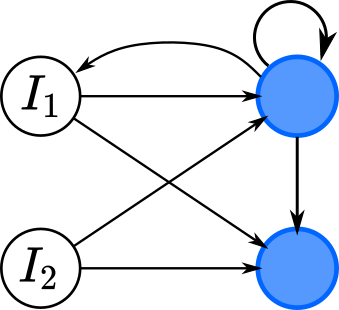
\includegraphics[scale=0.6]{figs/fibo2_ecoli.png}
    \caption{2-Fibonnaci Fiber $|\phi_2 = 1.6180..., \ell = 2\rangle$}
    \label{fig:fig4_l2}
\end{figure}

\subsection{Special model}

\begin{equation}
    \begin{aligned}
        f(u,v,I_1, I_2) &= -\alpha u + (1-S(v)) + I_1(v) + I_2\\
        g(u,v) &= -\delta u + \beta v
    \end{aligned}
\end{equation}
Here we need to decide the expression 
of $I_1(v)$. For instance, $I_1(v) = Iv$ 
with $I$ constant. In this case, we have 
$\nicefrac{\partial f}{\partial v} = -S'(v) + I = b$ 
at the equilibrium point.

In this case, $b > 0$ if $I < S'(v)$; 
$b < 0$ if $I > S'(v)$, and $b = 0$ if
$I = S'(v)$. Therefore, in this simple case
$I$ is a bifurcation parameter.

\section{2-Fibonacci Fiber on $| n = 1, \ell = 2\rangle$}

\begin{figure}[H]
    \centering
    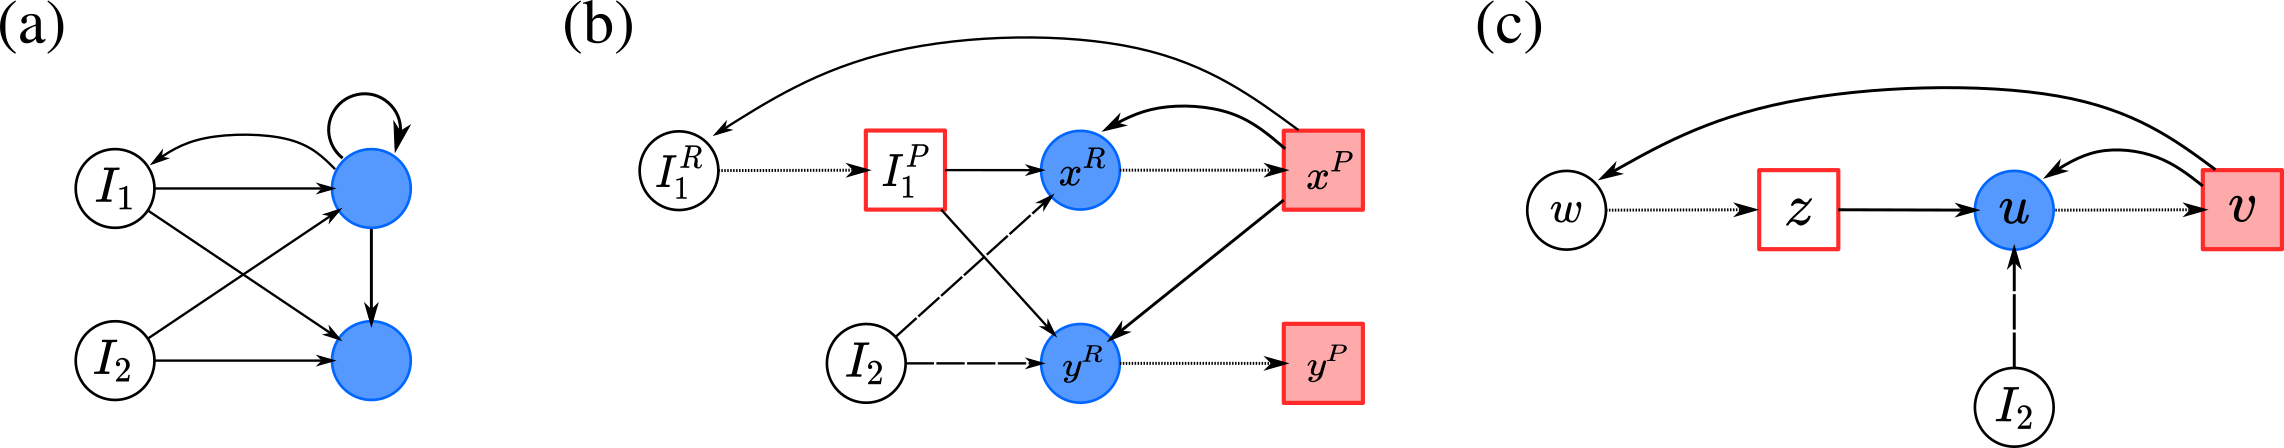
\includegraphics[scale=0.425]{figs/fibo2.png}
    \caption{(a) Biological representation, 
        (b) Mathematical representation, and (c) quotient
        network.}
    \label{fig:fig5}
\end{figure}

\subsection{General admissible equations}
\begin{equation} \label{eq:2fibo}
    \begin{aligned}
        \dot{x}^R &= f(x^R, x^P, I_1, I_2)\\
        \dot{x}^P &= g(x^P, x^R)\\
        \dot{y}^R &= f(y^R, x^P, I_1, I_2)\\
        \dot{y}^P &= g(y^P, y^R)\\
        \dot{I}_1^R &= f(I_1^R, x^P)\\
        \dot{I}_1^P &= g(I_1^P, I_1^R)
    \end{aligned}
\end{equation}
with vector of coordinates 
$\vec{x} = (x^R, x^P, y^R, y^P, I_1^R, I_1^P)$.

\subsection{Jacobian and eigenvalues}

Considering the partial derivatives obtained from 
Eq.~\ref{eq:2fibo}, we have:
$\nicefrac{\partial \dot{x}^R}{\partial {x}^R} = f_1$,
$\nicefrac{\partial \dot{x}^R}{\partial {x}^P} = f_2$,
$\nicefrac{\partial \dot{x}^R}{\partial {I_1}^P} = f_3$,
$\nicefrac{\partial \dot{x}^P}{\partial {x}^R} = g_2$,
$\nicefrac{\partial \dot{x}^P}{\partial {x}^P} = g_1$,
$\nicefrac{\partial \dot{y}^R}{\partial {x}^R} = f_1$,
$\nicefrac{\partial \dot{y}^R}{\partial {x}^P} = f_2$,
$\nicefrac{\partial \dot{y}^R}{\partial {I_1}^P} = f_3$,
$\nicefrac{\partial \dot{y}^P}{\partial {x}^P} = g_1$,
$\nicefrac{\partial \dot{y}^P}{\partial {y}^R} = g_2$,
$\nicefrac{\partial \dot{I_1}^R}{\partial {I_1}^R} = i_1$,
$\nicefrac{\partial \dot{I_1}^R}{\partial {x}^P} = i_2$,
$\nicefrac{\partial \dot{I_1}^P}{\partial {I_1}^R} = j_2$,
$\nicefrac{\partial \dot{I_1}^P}{\partial {I_1}^P} = j_1$.
From these derivatives at the equilibrium point, the 
Jacobian is given as
\begin{equation}
    J = \begin{pmatrix}
        f_1 & f_2 & 0 & 0 & f_3 & 0\\
        g_2 & g_1 & 0 & 0 & 0 & 0\\
        0 & f_2 & f_1 & 0 & f_3 & 0\\
        0 & 0 & g_2 & g_1 & 0 & 0\\
        0 & i_2 & 0 & 0 & i_1 & 0\\
        0 & 0 & 0 & 0 & j_2 & j_1\\
    \end{pmatrix}_{\big|_{eq.}} = 
    \begin{pmatrix}
        a & b & 0 & 0 & c & 0\\
        e & d & 0 & 0 & 0 & 0\\
        0 & b & a & 0 & c & 0\\
        0 & 0 & e & d & 0 & 0\\
        0 & q & 0 & 0 & p & 0\\
        0 & 0 & 0 & 0 & l & k\\
    \end{pmatrix}
\end{equation}

\end{document}